\begin{figure}[H]
\centering
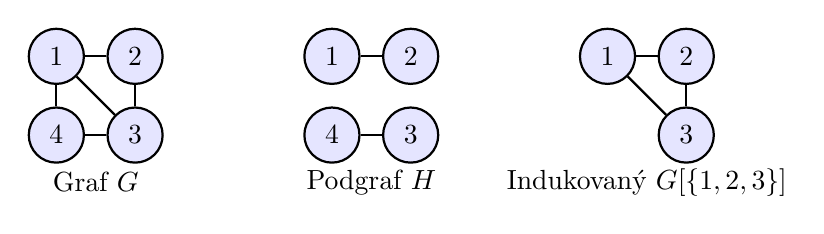
\begin{tikzpicture}[
  vnode/.style={circle, draw, minimum size=7mm, inner sep=0pt, fill=blue!10},
  thick
]
  % G
  \begin{scope}[shift={(0,0)}]
    \node[vnode] (1) at (0, 1) {1};
    \node[vnode] (2) at (1, 1) {2};
    \node[vnode] (3) at (1, 0) {3};
    \node[vnode] (4) at (0, 0) {4};
    \draw (1) -- (2);
    \draw (2) -- (3);
    \draw (3) -- (4);
    \draw (4) -- (1);
    \draw (1) -- (3);
    \node at (0.5, -0.6) {Graf $G$};
  \end{scope}
  
  % Podgraf H
  \begin{scope}[shift={(3.5,0)}]
    \node[vnode] (1') at (0, 1) {1};
    \node[vnode] (2') at (1, 1) {2};
    \node[vnode] (3') at (1, 0) {3};
    \node[vnode] (4') at (0, 0) {4};
    \draw (1') -- (2');
    \draw (3') -- (4');
    \node at (0.5, -0.6) {Podgraf $H$};
  \end{scope}
  
  % Indukovaný podgraf G[V'] pro V' = {1, 2, 3}
  \begin{scope}[shift={(7,0)}]
    \node[vnode] (1'') at (0, 1) {1};
    \node[vnode] (2'') at (1, 1) {2};
    \node[vnode] (3'') at (1, 0) {3};
    \draw (1'') -- (2'');
    \draw (2'') -- (3'');
    \draw (1'') -- (3'');
    \node at (0.5, -0.6) {Indukovaný $G[\{1,2,3\}]$};
  \end{scope}
\end{tikzpicture}
\caption{Příklad grafu $G$, jeho podgrafu $H$ (chybí některé hrany) a indukovaného podgrafu na množině vrcholů $\{1, 2, 3\}$ (obsahuje všechny dostupné vnitřní hrany).}
\end{figure}